% vim: set spell spelllang=en_us :

Table~\ref{tab:tfg_adsorption_descriptors} reports the crossed-parent and
GM-parent \ce{Pt10CO} results. Table~\ref{tab:tfg_bimetallic_adsorption_descriptors}
reports the binding, structural, and vibrational descriptors for the
crossed-parent \ce{Pt_xGe_{10-x}CO} series. The corresponding GM-parent Pt--Ge
data are given in Supporting
Table~\ref{tab:tfg_gm_bimetallic_adsorption_descriptors}.

\begin{table}[H]
\centering
\begin{singlespace}
\caption{Relative energies, \ce{CO} binding energies, and structural and
vibrational descriptors for the distinct \ce{Pt10CO} minima obtained from the
\ce{Pt5Ge5}-derived and global-minimum parent structures. Within each parent
geometry and multiplicity series, $\Delta E_0$ is measured relative to the
lowest carbonyl minimum in that series. Each $BE$ uses free singlet \ce{CO}
and the optimized bare \ce{Pt10} cluster with the same parent framework and
multiplicity as the corresponding carbonyl. Site labels identify the initial
Pt placements; labels separated by ``/'' denote placements that converge to
the same optimized minimum.}
\label{tab:tfg_adsorption_descriptors}
\renewcommand{\arraystretch}{0.92}
\begin{tabular}{cclcccc}
\toprule
{$\Delta E_0$ / eV} & {$2S+1$} & {Site} & {$BE$ / eV} &
{$r(\ce{Pt-C})$ / \si{\angstromunit}} & {$r(\ce{C-O})$ / \si{\angstromunit}} &
{$\nu(\ce{CO})$ / \si{\per\centi\metre}} \\
\midrule
\multicolumn{7}{l}{\textit{\ce{Pt5Ge5}-derived crossed-parent series}} \\
\multicolumn{7}{l}{\quad $2S+1=3$} \\
0.000 & 3 & 6    & -2.657 & 1.831 & 1.158 & 2020.0 \\
0.007 & 3 & 8/10 & -2.650 & 1.831 & 1.159 & 2012.4 \\
0.068 & 3 & 3/5  & -2.590 & 1.835 & 1.159 & 2014.3 \\
0.079 & 3 & 4    & -2.579 & 1.836 & 1.159 & 2013.0 \\
0.164 & 3 & 2    & -2.493 & 1.833 & 1.160 & 2005.9 \\
0.165 & 3 & 7    & -2.493 & 1.836 & 1.159 & 2016.0 \\
0.502 & 3 & 1/9  & -2.156 & 1.837 & 1.156 & 2033.7 \\
\multicolumn{7}{l}{\quad $2S+1=5$} \\
0.000 & 5 & 5/7  & -2.645 & 1.834 & 1.159 & 2012.5 \\
0.334 & 5 & 2/10 & -2.311 & 1.834 & 1.158 & 2017.1 \\
0.421 & 5 & 3/6  & -2.223 & 1.834 & 1.156 & 2032.6 \\
0.456 & 5 & 1/8  & -2.189 & 1.841 & 1.159 & 2011.0 \\
0.635 & 5 & 4/9  & -2.010 & 1.835 & 1.159 & 2006.3 \\
\midrule
\multicolumn{7}{l}{\textit{GM-parent series}} \\
\multicolumn{7}{l}{\quad $2S+1=5$} \\
0.000 & 5 & 3/6/9 & -2.275 & 1.820 & 1.158 & 2021.3 \\
0.049 & 5 & 1/2/8 & -2.226 & 1.819 & 1.159 & 2020.6 \\
0.670 & 5 & 7/10 & -1.605 & 1.876 & 1.155 & 2014.3 \\
0.709 & 5 & 5 & -1.566 & 1.876 & 1.156 & 2012.5 \\
0.728 & 5 & 4 & -1.547 & 1.877 & 1.156 & 2012.2 \\
\multicolumn{7}{l}{\quad $2S+1=7$} \\
0.000 & 7 & 8/9 & -2.353 & 1.820 & 1.159 & 2018.9 \\
0.000 & 7 & 1/2/3/6 & -2.353 & 1.820 & 1.159 & 2018.9 \\
0.598 & 7 & 4/5/7/10 & -1.755 & 1.877 & 1.155 & 2013.2 \\
\multicolumn{7}{l}{\quad $2S+1=9$} \\
0.000 & 9 & 1/2/3/6/8/9 & -1.595 & 1.857 & 1.156 & 2018.0 \\
0.015 & 9 & 4/5/7/10 & -1.580 & 1.888 & 1.155 & 2014.7 \\
\midrule
--- & 1 & free \ce{CO} & --- & --- & 1.137 & 2129.0 \\
\bottomrule
\end{tabular}
\end{singlespace}
\end{table}

\begin{table}[H]
\centering
\begin{singlespace}
\caption{\ce{CO} binding energies at the sampled Pt sites, together with
structural and vibrational descriptors, for the Ge-containing carbonyls
obtained from the crossed-parent models derived from the original \ce{Pt10}
framework. Rows are ordered by $BE$ within each composition. All carbonyls in
this table are singlets. Each $BE$ uses free singlet \ce{CO} and the isolated
bare crossed-parent cluster of the corresponding composition as references.
The corresponding global-minimum-parent data are reported separately in
Supporting Table~\ref{tab:tfg_gm_bimetallic_adsorption_descriptors}. Site
labels identify the initial Pt placements. Grouped labels denote positions
represented by the same optimized result, either because they are equivalent
in the parent structure or because they converge to the same minimum.}
\label{tab:tfg_bimetallic_adsorption_descriptors}
\renewcommand{\arraystretch}{0.92}
\begin{tabular}{lccccc}
\toprule
{Composition} &  {Site} & {$BE$ / eV} &
{$r(\ce{Pt-C})$ / \si{\angstromunit}} & {$r(\ce{C-O})$ / \si{\angstromunit}} &
{$\nu(\ce{CO})$ / \si{\per\centi\metre}} \\
\midrule
\ce{Pt6Ge4CO}  & 2    & -2.246 & 1.841 & 1.158 & 2019.21 \\
\ce{Pt6Ge4CO}  & 9    & -2.245 & 1.870 & 1.153 & 2037.50 \\
\ce{Pt6Ge4CO}  & 1/4  & -2.235 & 1.838 & 1.159 & 2018.43 \\
\ce{Pt6Ge4CO}  & 5/7    & -1.567 & 1.903 & 1.154 & 2018.58 \\
\midrule
\ce{Pt5Ge5CO}  & 6/8  & -2.076 & 1.895 & 1.157 & 2003.10 \\
\ce{Pt5Ge5CO}  & 7/10 & -1.661 & 1.888 & 1.154 & 2027.46 \\
\ce{Pt5Ge5CO}  & 4  & -1.342 & 1.924 & 1.156 & 2004.80 \\
\midrule
\ce{Pt4Ge6CO}  & 5/7 & -1.459 & 1.896 & 1.155 & 2019.36 \\
\ce{Pt4Ge6CO}  & 2 & -1.305 & 1.882 & 1.155 & 2020.88 \\
\ce{Pt4Ge6CO}  & 1 & -1.052 & 1.875 & 1.158 & 2004.13 \\
\bottomrule
\end{tabular}
\\
\end{singlespace}
\end{table}

Figure~\ref{fig:tfg_adsorption_distribution} summarizes the binding-energy
ranges and the mean values calculated from the data in the tables.

\begin{figure}[H]
\centering
\definecolor{ptten}{RGB}{35,35,35}
\definecolor{crossedparent}{RGB}{35,35,35}
\definecolor{globalparent}{RGB}{0,90,190}

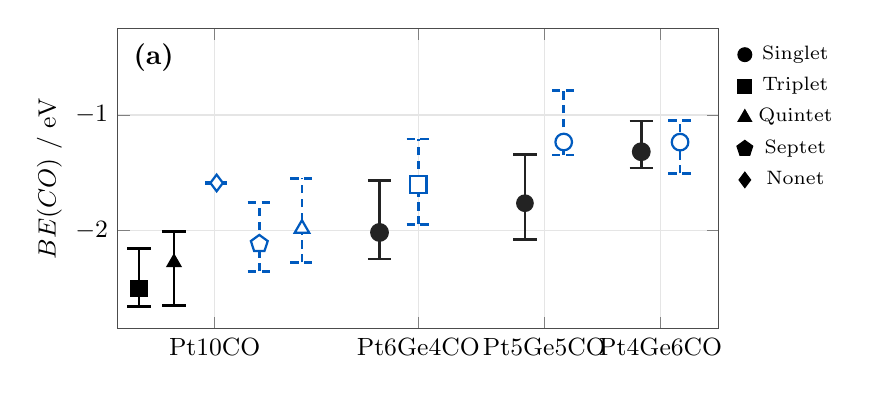
\begin{tikzpicture}
\begin{axis}[
  width=0.76\linewidth,
  height=5.4cm,
  xmin=0.45, xmax=3.55,
  ymin=-2.85, ymax=-0.25,
  xtick={0.95,2.00,2.65,3.25},
  xticklabels={\ce{Pt10CO},\ce{Pt6Ge4CO},\ce{Pt5Ge5CO},\ce{Pt4Ge6CO}},
  ylabel={$BE(\ce{CO})$ / eV},
  ylabel style={yshift=-2pt},
  tick label style={font=\small},
  label style={font=\small},
  grid=major,
  grid style={gray!20},
  axis line style={black!70},
  legend style={
    at={(1.02,0.98)},
    anchor=north west,
    draw=none,
    inner sep=2pt,
    row sep=1pt,
    font=\scriptsize,
    legend columns=1
  }
]
\addlegendimage{only marks,mark=*,mark size=2.5pt,black}
\addlegendentry{Singlet}
\addlegendimage{only marks,mark=square*,mark size=2.5pt,black}
\addlegendentry{Triplet}
\addlegendimage{only marks,mark=triangle*,mark size=2.8pt,black}
\addlegendentry{Quintet}
\addlegendimage{only marks,mark=pentagon*,mark size=3.0pt,black}
\addlegendentry{Septet}
\addlegendimage{only marks,mark=diamond*,mark size=2.8pt,black}
\addlegendentry{Nonet}
% Each vertical bar shows the minimum--maximum interval and each marker the
% mean over all Pt sites represented by the corresponding series. Horizontal
% offsets are used only for readability.
% Crossed-parent Pt10: triplet and quintet.
\addplot[ptten,line width=1.0pt] coordinates {(0.56,-2.657) (0.56,-2.156)};
\addplot[ptten,line width=1.0pt] coordinates {(0.50,-2.657) (0.62,-2.657)};
\addplot[ptten,line width=1.0pt] coordinates {(0.50,-2.156) (0.62,-2.156)};
\addplot[only marks,mark=square*,mark size=3.0pt,ptten] coordinates {(0.56,-2.501)};
\addplot[ptten,line width=1.0pt] coordinates {(0.74,-2.645) (0.74,-2.010)};
\addplot[ptten,line width=1.0pt] coordinates {(0.68,-2.645) (0.80,-2.645)};
\addplot[ptten,line width=1.0pt] coordinates {(0.68,-2.010) (0.80,-2.010)};
\addplot[only marks,mark=triangle*,mark size=3.0pt,ptten] coordinates {(0.74,-2.276)};
% Original Pt10 global-minimum parent: nonet, septet, and quintet.
\addplot[globalparent,densely dashed,line width=1.0pt] coordinates {(0.96,-1.595) (0.96,-1.580)};
\addplot[globalparent,densely dashed,line width=1.0pt] coordinates {(0.90,-1.595) (1.02,-1.595)};
\addplot[globalparent,densely dashed,line width=1.0pt] coordinates {(0.90,-1.580) (1.02,-1.580)};
\addplot[only marks,mark=diamond*,mark size=3.0pt,globalparent,
  mark options={fill=white,draw=globalparent,line width=0.8pt}] coordinates {(0.96,-1.588)};
\addplot[globalparent,densely dashed,line width=1.0pt] coordinates {(1.18,-2.353) (1.18,-1.755)};
\addplot[globalparent,densely dashed,line width=1.0pt] coordinates {(1.12,-2.353) (1.24,-2.353)};
\addplot[globalparent,densely dashed,line width=1.0pt] coordinates {(1.12,-1.755) (1.24,-1.755)};
\addplot[only marks,mark=pentagon*,mark size=3.2pt,globalparent,
  mark options={fill=white,draw=globalparent,line width=0.8pt}] coordinates {(1.18,-2.114)};
\addplot[globalparent,densely dashed,line width=1.0pt] coordinates {(1.40,-2.275) (1.40,-1.547)};
\addplot[globalparent,densely dashed,line width=1.0pt] coordinates {(1.34,-2.275) (1.46,-2.275)};
\addplot[globalparent,densely dashed,line width=1.0pt] coordinates {(1.34,-1.547) (1.46,-1.547)};
\addplot[only marks,mark=triangle*,mark size=3.0pt,globalparent,
  mark options={fill=white,draw=globalparent,line width=0.8pt}] coordinates {(1.40,-1.982)};
% Pt6Ge4: crossed-parent singlet and GM-parent triplet.
\addplot[crossedparent,line width=1.0pt] coordinates {(1.80,-2.246) (1.80,-1.567)};
\addplot[crossedparent,line width=1.0pt] coordinates {(1.74,-2.246) (1.86,-2.246)};
\addplot[crossedparent,line width=1.0pt] coordinates {(1.74,-1.567) (1.86,-1.567)};
\addplot[only marks,mark=*,mark size=3.2pt,crossedparent] coordinates {(1.80,-2.016)};
\addplot[globalparent,densely dashed,line width=1.0pt] coordinates {(2.00,-1.947) (2.00,-1.207)};
\addplot[globalparent,densely dashed,line width=1.0pt] coordinates {(1.94,-1.947) (2.06,-1.947)};
\addplot[globalparent,densely dashed,line width=1.0pt] coordinates {(1.94,-1.207) (2.06,-1.207)};
\addplot[
  only marks,mark=square*,mark size=3.0pt,globalparent,
  mark options={fill=white,draw=globalparent,line width=0.8pt}
] coordinates {(2.00,-1.600)};
% Pt5Ge5: crossed parent and GM parent.
\addplot[crossedparent,line width=1.0pt] coordinates {(2.55,-2.076) (2.55,-1.342)};
\addplot[crossedparent,line width=1.0pt] coordinates {(2.49,-2.076) (2.61,-2.076)};
\addplot[crossedparent,line width=1.0pt] coordinates {(2.49,-1.342) (2.61,-1.342)};
\addplot[only marks,mark=*,mark size=3.0pt,crossedparent] coordinates {(2.55,-1.763)};
\addplot[globalparent,densely dashed,line width=1.0pt] coordinates {(2.75,-1.346) (2.75,-0.788)};
\addplot[globalparent,densely dashed,line width=1.0pt] coordinates {(2.69,-1.346) (2.81,-1.346)};
\addplot[globalparent,densely dashed,line width=1.0pt] coordinates {(2.69,-0.788) (2.81,-0.788)};
\addplot[only marks,mark=*,mark size=3.0pt,globalparent,
  mark options={fill=white,draw=globalparent,line width=0.8pt}] coordinates {(2.75,-1.234)};
% Pt4Ge6: crossed parent and GM parent.
\addplot[crossedparent,line width=1.0pt] coordinates {(3.15,-1.459) (3.15,-1.052)};
\addplot[crossedparent,line width=1.0pt] coordinates {(3.09,-1.459) (3.21,-1.459)};
\addplot[crossedparent,line width=1.0pt] coordinates {(3.09,-1.052) (3.21,-1.052)};
\addplot[only marks,mark=*,mark size=3.2pt,crossedparent] coordinates {(3.15,-1.318)};
\addplot[globalparent,densely dashed,line width=1.0pt] coordinates {(3.35,-1.506) (3.35,-1.046)};
\addplot[globalparent,densely dashed,line width=1.0pt] coordinates {(3.29,-1.506) (3.41,-1.506)};
\addplot[globalparent,densely dashed,line width=1.0pt] coordinates {(3.29,-1.046) (3.41,-1.046)};
\addplot[only marks,mark=*,mark size=3.0pt,globalparent,
  mark options={fill=white,draw=globalparent,line width=0.8pt}] coordinates {(3.35,-1.235)};
\node[anchor=north west,font=\bfseries] at (rel axis cs:0.01,0.98) {(a)};
\end{axis}
\end{tikzpicture}

\caption{Distribution of \ce{CO} binding energies resolved by structural parent and
multiplicity. Solid black bars and filled black markers represent the
crossed-parent series. Dashed dark-blue bars and open dark-blue markers
represent series initiated from the corresponding global-minimum parent. Each
vertical segment spans the minimum--maximum
interval of one parent--multiplicity set, and the central symbol marks its
mean binding energy over all Pt sites represented in that set. A grouped site
label is weighted by the number of Pt positions that it contains, whether the
positions are equivalent in the parent or converge to the same final minimum.
Horizontal offsets within a composition are used only to avoid
overlap. Circles, squares, triangles, pentagons, and diamonds represent singlet,
triplet, quintet, septet, and nonet states, respectively.}
\label{fig:tfg_adsorption_distribution}
\end{figure}

{The triplet \ce{Pt10CO} data were obtained by replacing all Ge atoms in
the \ce{Pt5Ge5} framework with Pt before \ce{CO} adsorption.} They provide a
pure-Pt comparison shown alongside the
Pt--Ge composition series. The trajectory initiated at site 6 reaches the most strongly bound minimum,
whereas those initiated at sites 1 and 9 converge to the same weakest
minimum. The ten Pt sites give a mean binding energy of $-2.501$ eV, and the
seven unique minima span
$-2.657$ to $-2.156$ eV. Because the quintet state of bare \ce{Pt10} lies only 0.0413 eV
above the triplet, {we also calculated the quintet carbonyls to compare
the site-dependent adsorption patterns at these two nearby spin states.}
Counting the ten Pt sites, their mean is
$-2.276$ eV and their five unique minima span $-2.645$ to $-2.010$ eV.

{In the GM-parent \ce{Pt10CO} series, the nonet carbonyls bind weakly and
span a narrow range ($-1.595$ to $-1.580$ eV). The septet and quintet sets
span $-2.353$ to $-1.755$ eV and $-2.275$ to $-1.547$ eV, respectively.}

At the common quintet multiplicity, the two \(\ce{Pt10}\) parent structures provide a direct comparison of the effect of the initial framework. The \(\ce{Pt5Ge5}\)-derived quintet gives a mean binding energy of \(-2.276\) eV, whereas the quintet series initiated from the reported \(\ce{Pt10}\) global-minimum structure gives \(-1.983\) eV. Thus, within the same nominal spin state, the two parent structures differ by \(0.293\) eV in mean \(\ce{CO}\) binding energy. This result shows that the initial \(\ce{Pt10}\) framework can substantially change the sampled \(\ce{CO}\)-adsorption landscape.

Within the representative \ce{Pt10 -> Pt_xGe_{10-x}} crossed-parent sequence, the mean binding
energy over all Pt sites becomes progressively less negative from
\ce{Pt6Ge4CO} (-2.016 eV) to
\ce{Pt5Ge5CO} (-1.763 eV) and \ce{Pt4Ge6CO} (-1.318 eV). The corresponding
ranges are -2.246 to -1.567, -2.076 to -1.342, and -1.459 to -1.052 eV,
respectively. The site dependence remains appreciable, especially for
\ce{Pt5Ge5CO}, whose
values span 0.734 eV. Within this sequence, increasing the Ge content weakens
\ce{CO} adsorption on average, in agreement with earlier Pt--Ge
studies.\cite{ugartemendia:2021,ugartemendia:2022}

The GM-parent series for \ce{Pt_{x}Ge_{10-x}}, shown as dashed blue data in
Figure~\ref{fig:tfg_adsorption_distribution}, uses the spin state of the
bare-cluster GM for each composition. {This is the triplet for
\ce{Pt6Ge4} and the singlet for \ce{Pt5Ge5} and \ce{Pt4Ge6}.} For
\ce{Pt5Ge5CO}, the GM-parent series is shifted
substantially toward weaker adsorption and overlaps only marginally with the
crossed-parent range. The \ce{Pt4Ge6CO} GM-parent singlets cover a range
similar to the crossed-parent models, including both the most strongly and
most weakly bound structures. The \ce{Pt6Ge4CO} triplet GM-parent series spans
from $-1.947$ to $-1.207$~eV, with a mean of $-1.600$~eV.

Taken together,
these binding energies show that the crossed-parent series
gives a clear weakening of the representative \ce{CO} adsorption distributions as Ge
content increases,
but also that a given composition can show broad variation between Pt sites.
The GM-parent results also show that the calculated adsorption energies can
change by several tenths of an eV with the starting isomer and spin state.

\subsubsection{Local environment and structural response}

We next examine the local metal coordination around the Pt adsorption site,
the relation between the binding energy and the \ce{Pt-C} distance, and the
changes in the \ce{C-O} bond length and stretching frequency.

We also asked whether the relevant coordination of the adsorbing Pt atom
is simply its total number of metal neighbors, or whether the chemical
identity of those neighbors matters. For this purpose we used Hoppe's
effective coordination number, ECoN,\cite{hoppe:econ:1979} which replaces a hard distance cutoff by
smooth distance-dependent weights. {Short metal--metal contacts
contribute close to one, whereas longer contacts contribute progressively
less.} For a
center atom \(i\), each neighbor \(j\) is first described by the scaled
distance
\begin{equation}
s_{ij}=\frac{d_{ij}}{r_i^{\rm cov}+r_j^{\rm cov}},
\end{equation}
where \(d_{ij}\) is the distance between the two atoms and \(r^{\rm cov}\) are
covalent radii reported by Cordero et al.\cite{cordero:covalent-radii:2008}
For the metal atoms considered here, we used
\(r_{\ce{Pt}}=1.36~\si{\angstromunit}\) and \(r_{\ce{Ge}}=1.20~\si{\angstromunit}\).
Each neighbor then contributes with the weight
\begin{equation}
w_{ij}=\exp\left[1-\left(\frac{s_{ij}}{\bar{s}_i}\right)^6\right],
\end{equation}
and the effective coordination number is
\begin{equation}
ECoN_i=\sum_j w_{ij}.
\end{equation}
The reference distance \(\bar{s}_i\) is not fixed beforehand. It is the
weighted average of the same scaled distances,
\begin{equation}
\bar{s}_i=\frac{\sum_j s_{ij}w_{ij}}{\sum_j w_{ij}},
\end{equation}
so it is obtained iteratively until \(\bar{s}_i\) and the weights \(w_{ij}\)
are mutually consistent. In practice, this means that close neighbors
contribute almost as full contacts, whereas distant atoms contribute only
partially or negligibly. To characterize the environment encountered by
\ce{CO} before adsorption, the ECoN descriptors were calculated for each Pt
site in the corresponding bare parent structure. These quantities are denoted
by the superscript 0. Only metal neighbors were included. The same Hoppe
weights were partitioned according to the element of each neighbor, giving
$ECoN_{\rm total}^{0}=ECoN_{\rm Pt}^{0}+ECoN_{\rm Ge}^{0}$, and the Ge
contribution to the initial local environment was defined as
\begin{equation}
x_{\rm Ge}^{0}=\frac{ECoN_{\rm Ge}^{0}}{ECoN_{\rm total}^{0}}.
\end{equation}
For comparison, a superscript $\ce{CO}$ denotes a descriptor evaluated for
the optimized carbonyl structure, after adsorption and relaxation.
The pre-adsorption descriptors for the crossed-parent structures are
collected in Table~\ref{tab:tfg_crossed_ptge_econ_descriptors}. Calculating
them before CO is added avoids mixing the initial site environment with the
structural reorganization induced by adsorption. 
The corresponding descriptors calculated for
the GM parents are reported in Supporting
Table~\ref{tab:tfg_gm_ptge_econ_pre_descriptors} as a test of whether the
patterns found for the crossed-parent structures persist for a different
initial isomer.

For \ce{Pt6Ge4}, site 5/7 has the largest initial Ge fraction
($x_{\rm Ge}^{0}=0.809$) and gives the weakest CO binding in the series
($BE=-1.567$ eV). By contrast, sites 2 and 1/4 combine substantial effective
Pt coordination with smaller $x_{\rm Ge}^{0}$ values and give three of the
strongest binding energies. This comparison is consistent with weaker CO
binding as the Ge contribution to the initial Pt environment increases.
{Site 9 is an exception. Although its initial Ge fraction is relatively
large ($x_{\rm Ge}^{0}=0.751$), its binding energy ($-2.245$ eV) is nearly the same as}
those of sites 2 and 1/4. Upon adsorption, however, the local environment of
site 9 changes appreciably: $ECoN_{\rm Pt}^{0}=0.727$ increases to
$ECoN_{\rm Pt}^{\ce{CO}}=1.163$, while $x_{\rm Ge}^{0}=0.751$ decreases to
$x_{\rm Ge}^{\ce{CO}}=0.614$. The corresponding changes at site 5/7 are
smaller: $ECoN_{\rm Pt}$ increases from 0.529 to 0.657 and $x_{\rm Ge}$
decreases from 0.809 to 0.771. Thus, the optimized site-9 carbonyl has a larger
effective Pt contribution than its initial environment suggests. This local
{reorganization may help explain why site 9 departs from the initial
trend. However, these ECoN changes describe the final local environment and
do not quantify the energetic contribution of reorganization.} The initial
local composition therefore contributes to the observed pattern but does not
determine the binding energy by itself. The descriptors of the optimized
carbonyls are reported in Supporting
Table~\ref{tab:tfg_crossed_ptge_econ_co_descriptors}.

The $ECoN_{\rm Pt}^{0}$ and $ECoN_{\rm Ge}^{0}$ components, which measure the
effective contributions from neighboring Pt and Ge atoms, respectively,
provide complementary information for \ce{Pt5Ge5}.
Site 4, which gives the weakest adsorption in this composition, has
$x_{\rm Ge}^{0}\simeq1$ and essentially no effective Pt coordination. By
contrast, sites 6/8 and 7/10 have almost identical $x_{\rm Ge}^{0}$ values,
but their total effective coordination numbers differ markedly (about 5.58
and 2.91, respectively), together with a 0.42~eV difference in binding energy.
This difference in total coordination is largely retained after adsorption:
$ECoN_{\rm total}^{\ce{CO}}$ is 5.69 for site 6/8 and 2.95 for site 7/10,
increases of only 0.11 and 0.05, respectively. In both carbonyls,
$x_{\rm Ge}$ decreases ($0.745$ to $0.703$ for site 6/8 and $0.746$ to
$0.683$ for site 7/10), indicating a shift in the local coordination balance
toward Pt. Thus, the two sites retain very different total coordination after
CO adsorption despite having similar Ge fractions. This comparison describes
how their local environments change, but does not by itself explain the
0.42~eV difference in binding energy.

For \ce{Pt4Ge6}, all sampled sites are Ge-rich, but the pre-adsorption
descriptors clarify the weakest-binding structure. Site 1 has
$x_{\rm Ge}^{0}=0.980$ and $ECoN_{\rm Pt}^{0}=0.089$, showing that the
adsorbing Pt atom is initially almost completely coordinated by Ge. Sites 5
and 7 have different initial ECoN descriptors and are therefore listed
separately in Table~\ref{tab:tfg_crossed_ptge_econ_descriptors}, although both
adsorption trajectories converge to the same carbonyl minimum and give the
same binding energy. Together with site 2, they retain larger effective
contributions from Pt than site 1 and bind CO more strongly. Upon adsorption,
however, site 1 undergoes substantial local
reorganization: $ECoN_{\rm Pt}^{\ce{CO}}$ increases to 1.423 and
$x_{\rm Ge}^{\ce{CO}}$ falls to 0.759. The ECoN descriptors of the optimized
crossed-parent carbonyls are reported in Supporting
Table~\ref{tab:tfg_crossed_ptge_econ_co_descriptors}; the corresponding
final-state descriptors for the GM-parent structures are given in Supporting
Table~\ref{tab:tfg_gm_ptge_econ_descriptors}.

We next use the GM-parent series to examine whether the relation between the
initial Pt/Ge environment and CO binding found above persists when the starting
cluster isomer is changed. For \ce{Pt6Ge4}, the four sites with
$x_{\rm Ge}^{0}=0.337$--0.563 give the strongest triplet binding energies
($-1.947$ to $-1.657$~eV), whereas sites 4 and 5 have more Ge-rich initial
environments ($x_{\rm Ge}^{0}=0.807$ and 0.802) and give the weakest values
($-1.207$ and $-1.215$~eV). A similar distinction is found for \ce{Pt5Ge5}:
sites 1, 2, 4, and 5
have $x_{\rm Ge}^{0}=0.929$--0.930 and converge to the same carbonyl minimum,
whereas site 3 is almost completely coordinated by Ge
($x_{\rm Ge}^{0}=0.998$) and gives the weakest binding. The \ce{Pt4Ge6}
series is less regular. All four sites are Ge-rich. Sites 2 and 3 have similar
initial Ge fractions (0.920 and 0.905), yet they give the strongest and weakest
binding energies, respectively ($-1.506$ and $-1.046$ eV). {Thus, the
initial ECoN descriptors distinguish important features of the adsorption
environment, but they do not determine the complete binding-energy order.}

{Overall, the initial ECoN descriptors show that Pt sites with a larger
Ge contribution generally bind \ce{CO} less strongly.}
{The exception at site 9 of \ce{Pt6Ge4} and the variation across the
GM-parent \ce{Pt4Ge6} series show that ECoN describes the initial local
environment, but does not by itself determine the binding-energy order. We next examine the optimized Pt–C and C–O bond lengths and the CO stretching frequency to characterize the carbonyl after relaxation.}

\begin{table}[H]
\begin{center}
\caption{Local Hoppe ECoN descriptors for each Pt adsorption site in the bare
crossed-parent Pt--Ge clusters, before \ce{CO} is added. The superscript 0
denotes this pre-adsorption geometry. Only metal neighbors are included, and
$ECoN_{\rm total}^{0}=ECoN_{\rm Pt}^{0}+ECoN_{\rm Ge}^{0}$ and
$x_{\rm Ge}^{0}=ECoN_{\rm Ge}^{0}/ECoN_{\rm total}^{0}$. Paired labels denote
initial positions represented by the same listed descriptors and adsorption
result. Sites 5 and 7 of \ce{Pt4Ge6CO} are listed separately because their
initial ECoN descriptors differ, although they converge to the same carbonyl
minimum.}
\label{tab:tfg_crossed_ptge_econ_descriptors}
\small
\begin{tabular}{lcrrrrr}
\toprule
{System} &  {Site} & {$BE$ / eV} &
{$ECoN_{\rm total}^{0}$} & {$ECoN_{\rm Pt}^{0}$} & {$ECoN_{\rm Ge}^{0}$} &
{$x_{\rm Ge}^{0}$} \\
\midrule
\ce{Pt6Ge4CO}  & 2  & -2.246 & 3.222 & 1.882 & 1.339 & 0.416 \\
\ce{Pt6Ge4CO}  & 9  & -2.245 & 2.916 & 0.727 & 2.189 & 0.751 \\
\ce{Pt6Ge4CO}  & 1/4  & -2.235 & 4.596 & 2.696 & 1.900 & 0.413 \\
\ce{Pt6Ge4CO}  & 5/7  & -1.567 & 2.773 & 0.529 & 2.244 & 0.809 \\
\midrule
\ce{Pt5Ge5CO}  & 6/8  & -2.076 & 5.581 & 1.423 & 4.158 & 0.745 \\
\ce{Pt5Ge5CO}  & 7/10 & -1.661 & 2.905 & 0.738 & 2.168 & 0.746 \\
\ce{Pt5Ge5CO}  & 4  & -1.342 & 2.946 & 0.001 & 2.945 & 1.000 \\
\midrule
\ce{Pt4Ge6CO}  & 5  & -1.459 & 3.990 & 0.560 & 3.429 & 0.860 \\
\ce{Pt4Ge6CO}  & 7  & -1.459 & 3.480 & 0.281 & 3.199 & 0.919 \\
\ce{Pt4Ge6CO}  & 2  & -1.305 & 4.713 & 0.466 & 4.247 & 0.901 \\
\ce{Pt4Ge6CO}  & 1  & -1.052 & 4.407 & 0.089 & 4.317 & 0.980 \\
\bottomrule
\end{tabular}
\end{center}
\end{table}

\begin{figure}[H]
\centering
\definecolor{ptten}{RGB}{0,0,0}
\definecolor{ptsixgefour}{RGB}{0,114,178}
\definecolor{ptfivegefive}{RGB}{213,94,0}
\definecolor{ptfourgesix}{RGB}{0,158,115}

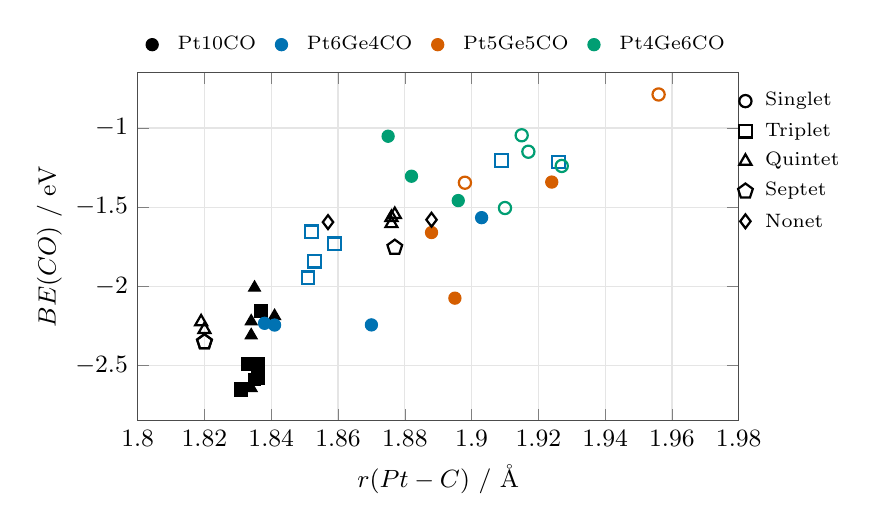
\begin{tikzpicture}
\begin{axis}[
  width=0.76\linewidth,
  height=6.0cm,
  xmin=1.80, xmax=1.98,
  ymin=-2.85, ymax=-0.65,
  xlabel={$r(\ce{Pt-C})$ / \AA},
  ylabel={$BE(\ce{CO})$ / eV},
  ylabel style={yshift=-2pt},
  tick label style={font=\small},
  label style={font=\small},
  grid=major,
  grid style={gray!20},
  axis line style={black!70},
  clip=false,
  legend style={at={(0.5,1.03)},anchor=south,draw=none,inner sep=1pt,
    font=\scriptsize,legend columns=4,column sep=5pt}
]
\addlegendimage{only marks,mark=*,mark size=2.2pt,ptten}
\addlegendentry{\ce{Pt10CO}}
\addlegendimage{only marks,mark=*,mark size=2.2pt,ptsixgefour}
\addlegendentry{\ce{Pt6Ge4CO}}
\addlegendimage{only marks,mark=*,mark size=2.2pt,ptfivegefive}
\addlegendentry{\ce{Pt5Ge5CO}}
\addlegendimage{only marks,mark=*,mark size=2.2pt,ptfourgesix}
\addlegendentry{\ce{Pt4Ge6CO}}
% Filled symbols: crossed-parent models.
\addplot[only marks,mark=square*,mark size=2.3pt,ptten] coordinates {
  (1.831,-2.657) (1.831,-2.650) (1.835,-2.590) (1.836,-2.579)
  (1.833,-2.493) (1.836,-2.493) (1.837,-2.156)};
\addplot[only marks,mark=triangle*,mark size=2.5pt,ptten] coordinates {
  (1.834,-2.645) (1.834,-2.311) (1.834,-2.223) (1.841,-2.189)
  (1.835,-2.010)};
\addplot[only marks,mark=*,mark size=2.2pt,ptsixgefour] coordinates {
  (1.841,-2.246) (1.870,-2.245) (1.838,-2.235) (1.903,-1.567)};
\addplot[only marks,mark=*,mark size=2.2pt,ptfivegefive] coordinates {
  (1.895,-2.076) (1.888,-1.661) (1.924,-1.342)};
\addplot[only marks,mark=*,mark size=2.2pt,ptfourgesix] coordinates {
  (1.896,-1.459) (1.882,-1.305) (1.875,-1.052)};
% Open symbols: models initiated from the global-minimum parent.
\addplot[only marks,mark=triangle,mark size=2.5pt,ptten,
  mark options={fill=white,draw=ptten,line width=0.8pt}] coordinates {
  (1.820,-2.275) (1.819,-2.226) (1.876,-1.605) (1.876,-1.566)
  (1.877,-1.547)};
\addplot[only marks,mark=pentagon,mark size=2.8pt,ptten,
  mark options={fill=white,draw=ptten,line width=0.8pt}] coordinates {
  (1.820,-2.353) (1.820,-2.353) (1.877,-1.755)};
\addplot[only marks,mark=diamond,mark size=2.5pt,ptten,
  mark options={fill=white,draw=ptten,line width=0.8pt}] coordinates {
  (1.857,-1.595) (1.888,-1.580)};
\addplot[only marks,mark=square,mark size=2.3pt,ptsixgefour,
  mark options={fill=white,draw=ptsixgefour,line width=0.8pt}] coordinates {
  (1.851,-1.947) (1.853,-1.842) (1.859,-1.732) (1.852,-1.657)
  (1.926,-1.215) (1.909,-1.207)};
\addplot[only marks,mark=o,mark size=2.2pt,ptfivegefive,
  mark options={fill=white,draw=ptfivegefive,line width=0.8pt}] coordinates {
  (1.898,-1.346) (1.956,-0.788)};
\addplot[only marks,mark=o,mark size=2.2pt,ptfourgesix,
  mark options={fill=white,draw=ptfourgesix,line width=0.8pt}] coordinates {
  (1.910,-1.506) (1.927,-1.240) (1.917,-1.150) (1.915,-1.046)};
% Symbol key: fill is reserved for the structural-parent distinction.
\addplot[only marks,mark=o,mark size=2.2pt,black,
  mark options={fill=white,draw=black,line width=0.8pt}] coordinates {(1.982,-0.83)};
\node[anchor=west,font=\scriptsize] at (axis cs:1.985,-0.83) {Singlet};
\addplot[only marks,mark=square,mark size=2.3pt,black,
  mark options={fill=white,draw=black,line width=0.8pt}] coordinates {(1.982,-1.02)};
\node[anchor=west,font=\scriptsize] at (axis cs:1.985,-1.02) {Triplet};
\addplot[only marks,mark=triangle,mark size=2.5pt,black,
  mark options={fill=white,draw=black,line width=0.8pt}] coordinates {(1.982,-1.21)};
\node[anchor=west,font=\scriptsize] at (axis cs:1.985,-1.21) {Quintet};
\addplot[only marks,mark=pentagon,mark size=2.8pt,black,
  mark options={fill=white,draw=black,line width=0.8pt}] coordinates {(1.982,-1.40)};
\node[anchor=west,font=\scriptsize] at (axis cs:1.985,-1.40) {Septet};
\addplot[only marks,mark=diamond,mark size=2.5pt,black,
  mark options={fill=white,draw=black,line width=0.8pt}] coordinates {(1.982,-1.59)};
\node[anchor=west,font=\scriptsize] at (axis cs:1.985,-1.59) {Nonet};
\end{axis}
\end{tikzpicture}

\caption{Binding energy versus the optimized \ce{Pt-C} distance for the
carbonyls. Black, blue, vermilion, and green identify \ce{Pt10CO},
\ce{Pt6Ge4CO}, \ce{Pt5Ge5CO}, and \ce{Pt4Ge6CO}, respectively. Filled symbols
denote crossed-parent structures and open symbols denote structures initiated
from the corresponding global-minimum parent. Circles, squares, triangles,
pentagons, and diamonds represent singlet, triplet, quintet, septet, and
nonet states, respectively.}
\label{fig:neutral_be_vs_ptc}
\end{figure}

\begin{figure}[H]
\centering
\definecolor{ptten}{RGB}{0,0,0}
\definecolor{ptsixgefour}{RGB}{0,114,178}
\definecolor{ptfivegefive}{RGB}{213,94,0}
\definecolor{ptfourgesix}{RGB}{0,158,115}

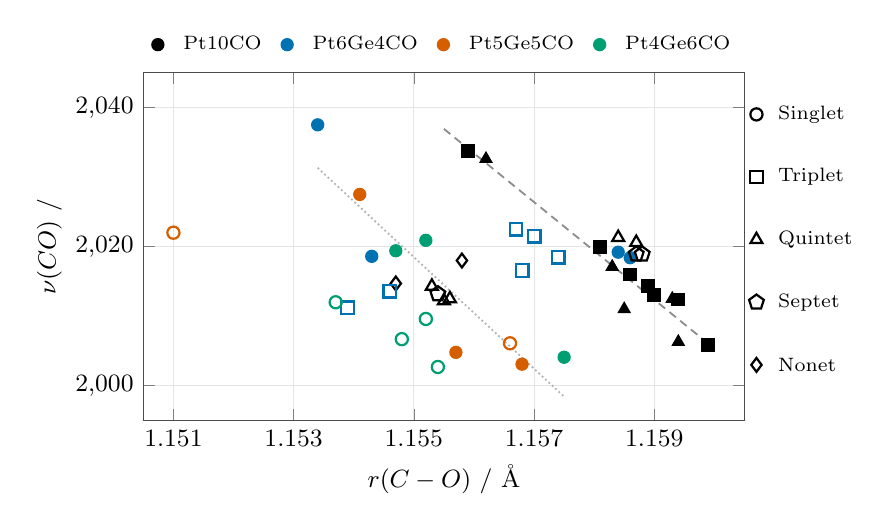
\begin{tikzpicture}
\begin{axis}[
  width=0.76\linewidth,
  height=6.0cm,
  xmin=1.1505, xmax=1.1605,
  ymin=1995, ymax=2045,
  xlabel={$r(\ce{C-O})$ / \AA},
  ylabel={$\nu(\ce{CO})$ / \si{\per\centi\metre}},
  ylabel style={yshift=-2pt},
  xtick={1.151,1.153,1.155,1.157,1.159},
  xticklabel style={/pgf/number format/fixed,/pgf/number format/precision=3},
  ytick={2000,2020,2040},
  tick label style={font=\small},
  label style={font=\small},
  grid=major,
  grid style={gray!20},
  axis line style={black!70},
  clip=false,
  legend style={at={(0.5,1.03)},anchor=south,draw=none,inner sep=1pt,
    font=\scriptsize,legend columns=4,column sep=5pt}
]
\addlegendimage{only marks,mark=*,mark size=2.2pt,ptten}
\addlegendentry{\ce{Pt10CO}}
\addlegendimage{only marks,mark=*,mark size=2.2pt,ptsixgefour}
\addlegendentry{\ce{Pt6Ge4CO}}
\addlegendimage{only marks,mark=*,mark size=2.2pt,ptfivegefive}
\addlegendentry{\ce{Pt5Ge5CO}}
\addlegendimage{only marks,mark=*,mark size=2.2pt,ptfourgesix}
\addlegendentry{\ce{Pt4Ge6CO}}
% Visual guides for the filled crossed-parent data sets only; no regression is implied.
\addplot[black!45,densely dashed,line width=0.65pt]
  coordinates {(1.15550,2036.92) (1.16000,2005.35)};
\addplot[gray!60,densely dotted,line width=0.65pt]
  coordinates {(1.15340,2031.32) (1.15750,1998.44)};
% Filled symbols: crossed-parent models.
\addplot[only marks,mark=square*,mark size=2.3pt,ptten] coordinates {
 (1.1581,2020.0) (1.1594,2012.4) (1.1589,2014.3) (1.1590,2013.0)
 (1.1599,2005.9) (1.1586,2016.0) (1.1559,2033.7)};
\addplot[only marks,mark=triangle*,mark size=2.5pt,ptten] coordinates {
 (1.1593,2012.5) (1.1583,2017.1) (1.1562,2032.6) (1.1585,2011.0)
 (1.1594,2006.3)};
\addplot[only marks,mark=*,mark size=2.2pt,ptsixgefour] coordinates {
 (1.1584,2019.2) (1.1534,2037.5) (1.1586,2018.4) (1.1543,2018.6)};
\addplot[only marks,mark=*,mark size=2.2pt,ptfivegefive] coordinates {
 (1.1568,2003.1) (1.1541,2027.5) (1.1557,2004.8)};
\addplot[only marks,mark=*,mark size=2.2pt,ptfourgesix] coordinates {
 (1.1547,2019.4) (1.1552,2020.9) (1.1575,2004.1)};
% Open symbols: models initiated from the global-minimum parent.
\addplot[only marks,mark=triangle,mark size=2.5pt,ptten,
  mark options={fill=white,draw=ptten,line width=0.8pt}] coordinates {
 (1.1584,2021.3) (1.1587,2020.6) (1.1553,2014.3) (1.1556,2012.5)
 (1.1555,2012.2)};
\addplot[only marks,mark=pentagon,mark size=2.8pt,ptten,
  mark options={fill=white,draw=ptten,line width=0.8pt}] coordinates {
 (1.1587,2018.9) (1.1588,2018.9) (1.1554,2013.2)};
\addplot[only marks,mark=diamond,mark size=2.5pt,ptten,
  mark options={fill=white,draw=ptten,line width=0.8pt}] coordinates {
 (1.1558,2018.0) (1.1547,2014.7)};
\addplot[only marks,mark=square,mark size=2.3pt,ptsixgefour,
  mark options={fill=white,draw=ptsixgefour,line width=0.8pt}] coordinates {
 (1.1574,2018.5) (1.1567,2022.5) (1.1568,2016.6) (1.1570,2021.5)
 (1.1539,2011.2) (1.1546,2013.6)};
\addplot[only marks,mark=o,mark size=2.2pt,ptfivegefive,
  mark options={fill=white,draw=ptfivegefive,line width=0.8pt}] coordinates {
 (1.1566,2006.1) (1.1510,2022.0)};
\addplot[only marks,mark=o,mark size=2.2pt,ptfourgesix,
  mark options={fill=white,draw=ptfourgesix,line width=0.8pt}] coordinates {
 (1.1552,2009.6) (1.1537,2012.0) (1.1548,2006.7) (1.1554,2002.7)};
% Symbol key: fill is reserved for the structural-parent distinction.
\addplot[only marks,mark=o,mark size=2.2pt,black,
  mark options={fill=white,draw=black,line width=0.8pt}] coordinates {(1.1607,2039)};
\node[anchor=west,font=\scriptsize] at (axis cs:1.1609,2039) {Singlet};
\addplot[only marks,mark=square,mark size=2.3pt,black,
  mark options={fill=white,draw=black,line width=0.8pt}] coordinates {(1.1607,2030)};
\node[anchor=west,font=\scriptsize] at (axis cs:1.1609,2030) {Triplet};
\addplot[only marks,mark=triangle,mark size=2.5pt,black,
  mark options={fill=white,draw=black,line width=0.8pt}] coordinates {(1.1607,2021)};
\node[anchor=west,font=\scriptsize] at (axis cs:1.1609,2021) {Quintet};
\addplot[only marks,mark=pentagon,mark size=2.8pt,black,
  mark options={fill=white,draw=black,line width=0.8pt}] coordinates {(1.1607,2012)};
\node[anchor=west,font=\scriptsize] at (axis cs:1.1609,2012) {Septet};
\addplot[only marks,mark=diamond,mark size=2.5pt,black,
  mark options={fill=white,draw=black,line width=0.8pt}] coordinates {(1.1607,2003)};
\node[anchor=west,font=\scriptsize] at (axis cs:1.1609,2003) {Nonet};
\end{axis}
\end{tikzpicture}

\caption{Harmonic \ce{C-O} stretching frequency versus the optimized
\ce{C-O} distance for the carbonyls. Black, blue, vermilion, and green identify
\ce{Pt10CO}, \ce{Pt6Ge4CO}, \ce{Pt5Ge5CO}, and \ce{Pt4Ge6CO}, respectively.
Filled symbols denote crossed-parent structures and open symbols denote
structures initiated from the corresponding global-minimum parent. Circles,
squares, triangles, pentagons, and diamonds represent singlet, triplet,
quintet, septet, and nonet states, respectively. The dashed black line is a
visual guide through the filled \ce{Pt10CO} triplet and quintet points. The
dotted gray line is a visual guide through the region occupied by most filled
Pt--Ge singlet points; it is not a regression line. The two filled
\ce{Pt6Ge4CO} structures initiated at site class 1/4 and site 2 fall clearly outside this
region.}
\label{fig:neutral_co_frequency}
\end{figure}

Figure~\ref{fig:neutral_be_vs_ptc} shows a broad trend, where shorter optimized
\ce{Pt-C} contacts generally correspond to more negative \ce{CO} binding
energies. The scatter, however, shows that the Pt--C distance alone does not
determine the adsorption energy.

For the crossed-parent \ce{Pt10CO}
series, the triplet minima have very similar \ce{Pt-C} distances,
1.830--1.837~\si{\angstromunit}, although their binding energies span about 0.50 eV (black
filled squares in
Figure~\ref{fig:neutral_be_vs_ptc}). The
\blue{Quintet minima (black filled triangles) show the same pattern. Their distances
cover only 1.834--1.841~\si{\angstromunit}, whereas their binding energies span
about 0.64 eV.} The GM-parent data (open symbols) extend the
range of \ce{Pt-C} distances, but they also involve different parent geometries
and spin states. Their broader scatter therefore reflects changes in more than
the \ce{Pt-C} distance alone.

The Pt--Ge carbonyls extend the sampled \ce{Pt-C} range to about
1.956~\si{\angstromunit}. Longer Pt--C contacts are often associated with weaker adsorption,
but this is not a strict relation for all structures. For example, the
\ce{Pt4Ge6CO} crossed-parent structures with similar \ce{Pt-C} distances have
binding energies that differ by several tenths of an eV. The local Pt/Ge
environment and relaxation of the whole cluster must therefore be considered
together with the Pt--C distance.

The internal \ce{C-O} bond connects this larger-cluster analysis with the
Blyholder interpretation used in earlier DFT studies.\cite{ugartemendia:2021,ugartemendia:2022} Within the
crossed-parent set, relative to free \ce{CO}, for which
$r(\ce{C-O})=1.137~\si{\angstromunit}$, the mean elongation is 0.022~\si{\angstromunit}{} for triplet
\ce{Pt10CO}. It decreases to 0.020, 0.019, and 0.019~\si{\angstromunit}{} for
\ce{Pt6Ge4CO}, \ce{Pt5Ge5CO}, and \ce{Pt4Ge6CO}, respectively. These
differences are small and individual structures are not strictly monotonic.
Even so, the predominant pattern indicates less activation of the \ce{C-O}
bond in the Ge-containing clusters. The small C--O changes are used here as a
complementary structural indicator. They agree with the previous DFT-based
NBO\cite{ugartemendia:2021} and PDOS\cite{ugartemendia:2022} analyses, and
are consistent with reduced metal-to-\ce{CO} back-donation upon Ge
substitution.

Figure~\ref{fig:neutral_co_frequency} shows the relation between the \ce{C-O}
bond length and stretching frequency for the crossed-parent and GM-parent
carbonyls. Badger's rule
relates the equilibrium bond length to the stretching force constant for the
same atomic pair.\cite{badger:1934,dabo:2012} The filled crossed-parent
\ce{Pt10CO} points show the expected inverse length--frequency pattern. Many
of the filled Pt--Ge singlet points occupy a second, distinct region of the
plot. The dashed black and dotted gray segments are included only as visual
guides to these two regions and are not regression lines. Two crossed-parent
\ce{Pt6Ge4CO} structures, initiated at site class 1/4 and site 2, lie clearly
outside the second region. They have the two longest \ce{C-O} bonds in this
subset (1.159 and 1.158~\si{\angstromunit}), but relatively low stretching
frequencies (2018.4 and 2019.2~\si{\per\centi\metre}). In their optimized structures, the
CO-binding Pt atom has one close Ge neighbor and two close Pt neighbors. This
more Pt-rich local environment is consistent with their stronger adsorption
and greater C--O activation. The global-minimum-parent points are distributed
over a wider part of the plot, both between and outside the two crossed-parent
regions. This broader distribution is observed for several compositions and
for the different \ce{Pt10} spin states, {showing that the distribution
also depends on the parent structure and spin state.}

Overall, the local descriptors give a consistent but incomplete picture.
Shorter \ce{Pt-C} distances and larger \ce{C-O} elongations generally accompany
stronger adsorption, and Ge-rich Pt environments tend to bind \ce{CO} more
weakly. The remaining scatter shows that these quantities must be read together
with the relaxation of the whole cluster, which is examined explicitly below.

\subsubsection{Interaction and fragment reorganization}
{To complement the ECoN analysis, we decompose the electronic adsorption
energy for selected strongly and weakly bound structures into the frozen-fragment
interaction and the metal and CO reorganization terms.}

The structural descriptors discussed above do not separate the direct
Pt--CO interaction from the energy associated with reorganizing the cluster
and \ce{CO}. To distinguish these contributions, we first compared two
triplet \ce{Pt10CO} minima obtained from the same \ce{Pt5Ge5 -> Pt10} parent:
the most strongly bound structure, initiated at site 6, and the weakest
minimum, reached from the site-1 and site-9 starting positions. Using the same
parent structure and multiplicity provides a direct comparison of the factors
responsible for their different binding energies. The electronic binding
energy contains both the Pt--CO interaction and the energy change caused by
reorganization of the two fragments. To separate these effects,
we first take the optimized \ce{Pt10CO} complex and remove \ce{CO} without
changing the coordinates of the metal cluster. This gives the frozen
\ce{Pt10} fragment, \(\mathbf R_{\ce{Pt10}}^{\ce{Pt10CO}}\). We do the
opposite for \ce{CO}, obtaining
\(\mathbf R_{\ce{CO}}^{\ce{Pt10CO}}\). The interaction energy is the energy
of the optimized complex minus the energies of these two frozen fragments:
\begin{align}
E_{\mathrm{int}} &=
E_{\ce{Pt10CO}}(\mathbf R_{\ce{Pt10CO}})
-E_{\ce{Pt10}}(\mathbf R_{\ce{Pt10}}^{\ce{Pt10CO}})
-E_{\ce{CO}}(\mathbf R_{\ce{CO}}^{\ce{Pt10CO}}),\\
E_{\mathrm{def}} &=
\left[
E_{\ce{Pt10}}(\mathbf R_{\ce{Pt10}}^{\ce{Pt10CO}})
-E_{\ce{Pt10}}(\mathbf R_{\ce{Pt10}}^{0})
\right]
{}+
\left[
E_{\ce{CO}}(\mathbf R_{\ce{CO}}^{\ce{Pt10CO}})
-E_{\ce{CO}}(\mathbf R_{\ce{CO}}^{0})
\right],
\label{eq:tfg_deformation}
\end{align}
Thus, $E_{\mathrm{int}}$ describes the electronic stabilization obtained when
the two frozen fragments are brought together at the geometry of the complex.
The deformation term in Eq.~\ref{eq:tfg_deformation} then measures what is
lost or gained by changing each isolated fragment from its own optimized
geometry, \(\mathbf R^0\), to the geometry it has in the complex. The first
bracket is the \ce{Pt10} contribution and the second is the \ce{CO}
contribution. Thus, $E_{\mathrm{def}}$ is the geometric cost, or benefit, of
preparing the two fragments for adsorption. A positive value is a deformation penalty; a negative value
means that the fragment geometry taken from the complex is more stable than
the isolated reference used here. The two bracketed terms are reported in
Table~\ref{tab:tfg_interaction_deformation} as
$E_{\rm reorg}^{\rm metal}$ and $E_{\rm reorg}^{\ce{CO}}$, respectively;
therefore,
$\Delta E_{\mathrm{elec}}=E_{\mathrm{int}}+E_{\mathrm{def}}$, where
$\Delta E_{\mathrm{elec}}$ is the electronic contribution to the binding
energy before the zero-point vibrational correction. The zero-point correction
is then added to obtain the final $BE$.


For the trajectory initiated at site 6, \(E_{\rm int}=-2.707\) eV. The
metal-cluster and \ce{CO} contributions to \(E_{\rm def}\) are \(-0.059\) eV
and \(+0.025\) eV, respectively. The first value shows that reorganization of
the \ce{Pt10} framework slightly strengthens the binding. The second is the
small energy cost of deforming \ce{CO}. Together, these terms give
\(E_{\rm def}=-0.034\) eV and \(\Delta E_{\rm elec}=-2.740\) eV.

For the weaker site-1/site-9 minimum, \(E_{\rm int}=-2.457\) eV. The
metal-cluster and \ce{CO} contributions are \(+0.201\) and \(+0.021\) eV,
respectively, giving \(E_{\rm def}=+0.221\) eV and
\(\Delta E_{\rm elec}=-2.235\) eV. The site-6 Pt--CO interaction is therefore
0.250 eV more stabilizing. In addition, the metal-framework contribution
changes from a \(+0.201\) eV penalty to a \(-0.059\) eV stabilization. These
differences account for most of the 0.505 eV difference in
\(\Delta E_{\rm elec}\). The complete decomposition and the corresponding
\(BE\) values are reported in
Table~\ref{tab:tfg_interaction_deformation}.

{This favorable metal contribution is consistent with the fragment
relaxation. After \ce{CO} is removed and the metal framework is reoptimized,
the cluster reaches another stable triplet minimum. Its $E_0$ lies 0.151 eV
below that of the initial \ce{Pt10} isomer. This result shows that adsorption
at site 6 can lead to reorganization of \ce{Pt10} toward a lower-energy
triplet isomer. The binding energy therefore includes both the
frozen-fragment interaction and a favorable change in the metal framework.}

{The same frozen-fragment analysis was then applied to representative strongly
and weakly bound minima in the crossed-parent \ce{Pt6Ge4CO}, \ce{Pt5Ge5CO},
and \ce{Pt4Ge6CO} series. For \ce{Pt6Ge4}, the stronger site has a much more
stabilizing interaction energy ($-2.704$ versus $-1.911$ eV). Its
metal-reorganization penalty is slightly larger (+0.345 versus +0.265 eV),
but this difference is too small to overcome the interaction advantage. Both
terms favor the stronger \ce{Pt4Ge6} site. Its interaction energy is
$-1.890$ eV, compared with $-1.664$ eV for site 1, and its metal
reorganization is smaller ($+0.341$ versus $+0.516$ eV).}

{The two \ce{Pt5Ge5} minima show a different balance. The strongly bound
site-6/8 structure has a less stabilizing frozen-fragment interaction than
site 4 ($-1.776$ versus $-1.920$ eV). However, its metal contribution is
favorable ($-0.396$ eV), whereas site 4 has a substantial reorganization
penalty ($+0.486$ eV). The different response of the metal framework therefore
reverses the ordering expected from $E_{\rm int}$ alone and gives the
site-6/8 carbonyl the more negative binding energy. {The negative metal
term means that the isolated \ce{Pt5Ge5} fragment at the geometry it adopts in
the site-6/8 carbonyl is 0.396 eV lower in energy than the isolated parent
reference. Thus, the binding energy includes stabilization of the metal
framework as it adopts the carbonyl geometry.} Thus, the crossed-parent series
shows that a strong \ce{CO} binding energy can arise either from a more
{favorable frozen-fragment interaction}, as in \ce{Pt6Ge4} and \ce{Pt4Ge6}, or from a
favorable structural response, as in \ce{Pt5Ge5}.}

\begin{table}[H]
\begin{center}
\caption{{Interaction and fragment-reorganization terms for selected strong
and weak \ce{CO}-binding minima obtained from the crossed-parent models. All
decomposed terms use electronic energies and are reported in eV. The \ce{Pt10}
entries are triplets and the \ce{Pt--Ge} entries are singlets. Each
isolated-cluster reference has the parent geometry and multiplicity used for
the corresponding binding energy. The final $BE$ column includes the
zero-point correction. The negative metal term for the \ce{Pt10} site-6
trajectory reflects relaxation toward a lower \ce{Pt10} isomer.}}
\label{tab:tfg_interaction_deformation}
%\scriptsize
\begin{tabular}{lclrrrrr}
\toprule
{System} & {$2S+1$} & {Site(s)} & {$\Delta E_{\rm elec}$} &
{$E_{\rm int}$} & {$E_{\rm reorg}^{\rm metal}$} &
{$E_{\rm reorg}^{\ce{CO}}$} & {$BE$} \\
\midrule
\ce{Pt10} & 3 & 6   & -2.740 & -2.707 & -0.059 & 0.025 & -2.657 \\
\ce{Pt10} & 3 & 1/9 & -2.235 & -2.457 &  0.201 & 0.021 & -2.156 \\
\midrule
\ce{Pt6Ge4} & 1 & 2   & -2.333 & -2.704 &  0.345 & 0.026 & -2.246 \\
\ce{Pt6Ge4} & 1 & 5/7 & -1.628 & -1.911 &  0.265 & 0.017 & -1.567 \\
\midrule
\ce{Pt5Ge5} & 1 & 6/8 & -2.149 & -1.776 & -0.396 & 0.023 & -2.076 \\
\ce{Pt5Ge5} & 1 & 4   & -1.414 & -1.920 &  0.486 & 0.020 & -1.342 \\
\midrule
\ce{Pt4Ge6} & 1 & 5/7 & -1.531 & -1.890 &  0.341 & 0.018 & -1.459 \\
\ce{Pt4Ge6} & 1 & 1   & -1.124 & -1.664 &  0.516 & 0.024 & -1.052 \\
\bottomrule
\end{tabular}

\medskip
\parbox{0.94\linewidth}{\footnotesize
After removal of CO from the site-6 complex, full relaxation gives another
triplet minimum with $E_{\rm elec}=-1194.30034094$~$E_h$ and
ZPVE $=0.006430$~$E_h$. It lies 0.151~eV below the orbital-stable
\ce{Pt5Ge5}-parent isomer used as the adsorption reference when zero-point
energies are included. {This result shows reorganization toward a
lower-energy isomer following \ce{CO} adsorption.}}
\end{center}
\end{table}

{Overall, the crossed-parent results show that the final \ce{CO} binding
energy is a balance between the \blue{frozen-fragment interaction} and the
structural response of the cluster. \blue{The frozen-fragment interaction} and metal
reorganization act in the same direction for the selected \ce{Pt4Ge6} sites. For
\ce{Pt6Ge4}, the \blue{frozen-fragment interaction} favors the stronger carbonyl, while the
larger reorganization penalty partly reduces this advantage. Their competition
determines the ordering of the selected \ce{Pt5Ge5} minima. Thus,
$E_{\mathrm{int}}$ alone does not define the binding energy, because relaxation
of the metal framework can reduce or reverse the interaction-based ordering.}
